\section{1ª Iteración}\label{cap:1_iteracion}

\subsection{Analisís}

\subsection{Diseño}

Antes de comenzar la implementación de esta primera iteración ha sido necesario tomar una serie de decisiones de diseño que condicionan el resto del proyecto: qué tecnologías se van a usar, cómo se organiza el código, cómo se guardan los datos y qué soluciones ya conocidas (patrones de diseño) conviene aplicar. Estas decisiones se explican a continuación con el detalle suficiente para que puedan entenderse sin conocimientos previos de React Native o Firebase, ya que sientan la base para el resto de iteraciones del proyecto.

\subsubsection{Decisiones tecnológicas}

Para el cliente\footnote{Cliente: en una arquitectura cliente-servidor, es la parte del sistema con la que interactúa directamente el usuario; en este caso, la propia aplicación instalada en el teléfono móvil.} móvil se ha optado por \textbf{React Native} \cite{reactnative}, un \emph{framework}\footnote{Framework: conjunto de herramientas y bibliotecas de código que facilitan el desarrollo de un tipo concreto de aplicación, proporcionando una estructura base sobre la que trabajar.} que permite escribir una única aplicación y ejecutarla tanto en Android como en iOS, en lugar de programar dos aplicaciones nativas independientes (una en Kotlin/Java para Android y otra en Swift para iOS). Se descarta el desarrollo nativo duplicado por dos motivos: el requisito RNF-07 exige que la aplicación funcione en ambas plataformas, y al tratarse de un proyecto desarrollado por una única persona, mantener y probar dos bases de código distintas multiplicaría el tiempo de desarrollo sin aportar ninguna ventaja funcional. Además, React Native dispone de librerías ya probadas para los dos puntos más críticos del sistema: la integración con mapas (\texttt{react-native-maps}) y el acceso a la geolocalización del dispositivo (\texttt{expo-location} o \texttt{react-native-geolocation-service}).

Como \emph{backend}\footnote{Backend: la parte del sistema que no ve el usuario directamente, encargada de almacenar los datos, gestionar la lógica de negocio y responder a las peticiones que le hace el cliente.} se ha optado por \textbf{Firebase} \cite{firebase}, una plataforma de Google que se ofrece como \emph{Backend-as-a-Service} (BaaS): en lugar de programar un servidor propio, se contratan una serie de servicios ya construidos (base de datos, autenticación de usuarios, almacenamiento de ficheros, envío de notificaciones) a los que la aplicación se conecta directamente. Se descarta programar un backend a medida porque Firebase ya resuelve de forma nativa todo lo anterior y, sobre todo, porque su base de datos (Cloud Firestore \cite{firestore}) permite que varios dispositivos vean los mismos datos actualizados en tiempo real sin que el equipo de desarrollo tenga que programar esa sincronización a mano: la aplicación simplemente se ``suscribe'' a los datos que le interesan y Firebase le avisa automáticamente cada vez que cambian (este mecanismo se denomina \emph{listener}, y se explica con más detalle en el apartado de patrones de diseño). Esta decisión es coherente con el riesgo ``Problemas con Firebase/base de datos'' identificado en la planificación (Sección~\ref{cap:analisisRiesgos}) y con el requisito RNF-08, que exige actualizar la posición de una procesión cada 30 segundos como mínimo.

Para los mapas se mantiene \textbf{Google Maps Platform} \cite{googlemapsapi}, ya justificado en el estado de la cuestión (Sección~1.3.2), por ser la solución de mapas más extendida y con mejor documentación. La contingencia prevista ante el riesgo ``Problemas con la integración de Google Maps'' (Sección~\ref{cap:analisisRiesgos}) sigue siendo migrar a OpenStreetMap \cite{openstreetmap} o Mapbox si en la práctica surgen problemas de cuota o de coste.

\subsubsection{Arquitectura del sistema}

La arquitectura de un sistema describe, a grandes rasgos, en qué piezas se divide y cómo se comunican entre sí. En este proyecto se ha definido una arquitectura \textbf{cliente-servidor sin servidor intermedio propio}: la aplicación React Native (el cliente) se comunica directamente con los SDK\footnote{SDK (\emph{Software Development Kit}): conjunto de herramientas que proporciona un servicio (en este caso, Firebase o Google Maps) para que otras aplicaciones puedan integrarse con él fácilmente, sin tener que hablar directamente con sus servidores a bajo nivel.} oficiales de Firebase (Authentication, Cloud Firestore, Cloud Messaging y Storage) y de Google Maps Platform (Maps SDK y Directions API). Es importante notar que no existe una capa de API REST\footnote{API REST: forma habitual de comunicación entre un cliente y un servidor propio, en la que el cliente pide o envía datos a través de peticiones HTTP a unas direcciones (\emph{endpoints}) definidas por el propio equipo de desarrollo. Al no tener servidor propio, esta capa no es necesaria en este proyecto.} propia entre el cliente y el servidor, como sí ocurriría si se hubiese optado por programar un backend a medida: es Firebase quien ya expone esa comunicación a través de su SDK. Internamente, el SDK de Firebase abre un canal de comunicación permanente con los servidores de Google (una conexión en tiempo real basada en HTTP/2, la misma tecnología que usa HTTPS) por la que viajan tanto las peticiones de lectura y escritura como los avisos de los \emph{listeners}; el SDK de Google Maps Platform, en cambio, solo se comunica puntualmente mediante peticiones HTTPS convencionales (por ejemplo, al calcular una ruta con la Directions API). En ambos casos es el propio SDK quien gestiona la conexión, la autenticación y la reconexión ante una pérdida de red, sin que la aplicación tenga que programar nada de eso.

\paragraph{Estructura del front-end}

Dentro del propio cliente, el código se organiza siguiendo una \textbf{arquitectura en capas} \cite{sommerville2015}: el proyecto se divide en varios grupos de carpetas (o \emph{paquetes}), cada uno con una responsabilidad concreta, de forma que cada capa solo puede depender de la capa inmediatamente inferior y nunca al revés. Esta regla se sigue para que un cambio en una capa concreta (por ejemplo, cambiar de Firebase a otro proveedor de datos) afecte al menor número posible de partes del código, y para poder probar cada capa de forma aislada. Las cuatro capas definidas son:

\begin{itemize}
    \item \textbf{UI} (\texttt{screens}, \texttt{components}, \texttt{navigation}): las pantallas que ve el usuario, agrupadas por su rol (ciudadano, cofrade, junta de cofradías, administrador), siguiendo los cuatro diagramas de casos de uso del Capítulo~\ref{cap:analisis}; los componentes visuales reutilizables entre pantallas (por ejemplo, la tarjeta con la información de una cofradía); y la navegación entre pantallas.
    \item \textbf{Application} (\texttt{context}, \texttt{hooks}): el estado que se comparte entre varias pantallas a la vez, como la sesión del usuario, su rol activo, la ciudad seleccionada o si está compartiendo su ubicación en ese momento.
    \item \textbf{Data} (\texttt{services}, \texttt{models}): un servicio por cada tipo de información del dominio (\texttt{cofradiaService}, \texttt{procesionService}, \texttt{geoService}, \texttt{notificationService}...) que es el único responsable de hablar con Firebase y con Google Maps, además de los tipos de datos que describen cómo es cada objeto (una cofradía, una procesión...) dentro de la aplicación.
    \item \textbf{Infrastructure} (\texttt{firebase}, \texttt{maps}): la configuración e inicialización de los SDK externos, es decir, el código mínimo necesario para que el resto de la aplicación pueda empezar a usar Firebase y Google Maps.
\end{itemize}

La Figura~\ref{fig:disenoPaquetes} muestra esta organización en forma de diagrama de paquetes, donde las flechas discontinuas indican qué paquete depende de (necesita) cuál.

\begin{figure}[H]
    \centering
    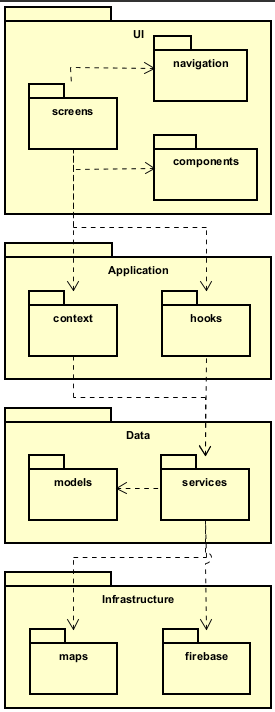
\includegraphics[width=0.45\textwidth]{imagenes/Dragrama de aplicacion front-end.png}
    \caption{Diagrama de paquetes de la aplicación cliente}
    \label{fig:disenoPaquetes}
\end{figure}

\paragraph{Estructura del back-end}

Como se ha explicado, el back-end de este proyecto no incluye código propio, sino que se apoya íntegramente en los siguientes servicios de Firebase:

\begin{itemize}
    \item \textbf{Firebase Authentication}: servicio que crea y gestiona la sesión de los usuarios con un rol elevado (cofrade, junta de cofradías, administrador), sin que el proyecto tenga que programar ni almacenar contraseñas por su cuenta. El ciudadano no necesita registrarse ni iniciar sesión en ningún momento: puede consultar procesiones, ver el mapa y recibir notificaciones sin tener ningún tipo de cuenta. Solo cuando un usuario introduce un código de acceso válido (colección \texttt{codigosAcceso}, ver apartado \nameref{sec:disenoBD}) se crea su sesión de Firebase Authentication y se le asigna el rol correspondiente.
    \item \textbf{Cloud Firestore}: la base de datos del proyecto. Guarda toda la información en las colecciones \texttt{ciudades}, \texttt{cofradias}, \texttt{eventos}, \texttt{procesiones}, \texttt{recorridos}, \texttt{usuarios} y \texttt{notificaciones} (el diseño completo de estas colecciones se explica en el apartado \nameref{sec:disenoBD} de esta misma sección).
    \item \textbf{Firebase Storage}: espacio de almacenamiento en la nube donde se guardan las imágenes de los pasos de cada cofradía, ya que este tipo de archivo no se guarda de forma eficiente dentro de la base de datos.
    \item \textbf{Cloud Messaging} \cite{firebasefcm}: servicio que permite enviar notificaciones \emph{push} (avisos que llegan al teléfono del usuario aunque no tenga la aplicación abierta en ese momento), usado para las alertas y avisos que publican las Juntas de Cofradías (RF-13, RF-14, RF-27).
\end{itemize}

\paragraph{Diagrama de despliegue}

Un diagrama de despliegue representa, de forma física, dónde se ejecuta cada parte del sistema y cómo se comunican entre sí esos entornos. La Figura~\ref{fig:disenoDespliegue} recoge el despliegue completo de este proyecto: el dispositivo móvil ejecuta la aplicación React Native, que se comunica mediante el protocolo HTTPS\footnote{HTTPS: versión segura (cifrada) del protocolo HTTP, usado habitualmente para la comunicación entre aplicaciones y servicios en internet.} tanto con Firebase (autenticación, base de datos, almacenamiento y notificaciones) como con Google Maps Platform (visualización de mapas y cálculo de rutas). Puede observarse que no existe ningún nodo de base de datos local: el requisito RNF-03 (disponibilidad de la información estática sin conexión a internet) queda cubierto por la caché\footnote{Caché: copia local y temporal de unos datos, guardada en el propio dispositivo, que permite seguir accediendo a ellos aunque se pierda la conexión a internet.} que Cloud Firestore guarda automáticamente en el dispositivo, sin que sea necesario implementar una base de datos local adicional como haría, por ejemplo, una aplicación Android nativa con Room. Este enfoque es más sencillo que el que sigue otro TFG de la escuela centrado en el funcionamiento sin conexión, el de Llorente Pérez~\cite{marioTFG}: su aplicación permite completar toda una actividad sin conexión a internet, guardando los datos en el propio dispositivo hasta poder enviarlos más tarde, porque está pensada para practicarse en el medio natural, donde puede no haber cobertura durante horas. En este proyecto, en cambio, las procesiones de Semana Santa transcurren en entornos urbanos con cobertura de red prácticamente garantizada, por lo que no hace falta un mecanismo tan complejo: basta con que la información estática (RNF-03) quede disponible sin conexión, que es justo lo que ya ofrece la caché de Firestore.

\begin{figure}[H]
    \centering
    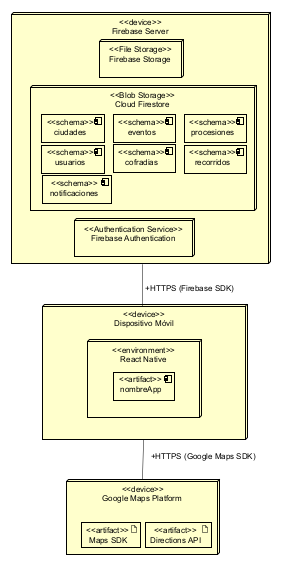
\includegraphics[width=0.45\textwidth]{imagenes/Diagrama de despliegue.png}
    \caption{Diagrama de despliegue de la aplicación}
    \label{fig:disenoDespliegue}
\end{figure}

\subsubsection{Diseño de la base de datos}\label{sec:disenoBD}

A diferencia de una base de datos relacional tradicional (como MySQL), organizada en tablas con filas y columnas relacionadas mediante claves, Cloud Firestore es una base de datos \textbf{NoSQL} \cite{nosql}\footnote{NoSQL: familia de bases de datos que no organiza la información en tablas relacionadas, sino en otras estructuras --en este caso, documentos agrupados en colecciones-- más flexibles para datos que cambian de forma o que se leen con mucha frecuencia en tiempo real.} de tipo documental: la información se organiza en \emph{colecciones} (agrupaciones de elementos del mismo tipo, similar a una carpeta) que contienen \emph{documentos} (cada elemento individual, similar a un fichero, con sus propios campos de datos). El modelo de dominio de la Figura~\ref{fig:DiagramDomain} se ha traducido a esta estructura de colecciones y subcolecciones (colecciones anidadas dentro de un documento concreto) siguiendo estas decisiones:

\begin{itemize}
    \item \texttt{pasos} y \texttt{puntosRuta} se modelan como \textbf{subcolecciones} de \texttt{cofradias} y \texttt{recorridos} respectivamente, porque siempre se consultan junto a su documento padre (por ejemplo, los pasos de una cofradía concreta) y nunca de forma independiente.
    \item \texttt{posicionActual} se modela como una \textbf{subcolección con un único documento} (\texttt{procesiones/\{id\}/posicionActual/actual}) en lugar de como un campo dentro del propio documento de la procesión, para que estas escrituras frecuentes de posición no afecten a los datos más estables de la procesión (horario, recorrido, pasos), que rara vez cambian. Este documento se sobrescribe cada vez que llega una nueva posición GPS. Cuando varios cofrades comparten su ubicación simultáneamente durante la misma procesión, sus posiciones se agregan y se escriben en modo \emph{batch} sobre este documento único, en lugar de realizar una escritura independiente por cada actualización individual, reduciendo así el número de operaciones sobre Firestore y, con ello, el consumo de ancho de banda y el coste asociado. El cliente se suscribe a este documento mediante un \emph{listener} en tiempo real (en vez de estar preguntando repetidamente si hay novedades, es Firestore quien avisa a la aplicación en cuanto el documento cambia), cumpliendo el requisito RNF-08 sin necesidad de implementar servidores de sockets propios. Al tratarse de un único documento por procesión que se sobrescribe con la posición agregada, el cliente recibe una sola actualización por cambio de posición en lugar de un flujo continuo de actualizaciones parciales por cada cofrade, evitando así problemas de parpadeo o sobrecarga en el mapa.
    \item \texttt{favoritos} no se guarda en Firestore, sino de forma local en el propio dispositivo (por ejemplo, con \texttt{AsyncStorage}), ya que el ciudadano no tiene cuenta ni sesión en la que persistir esta información en el servidor; únicamente se guarda el identificador de la cofradía o procesión marcada como favorita.
    \item \texttt{codigosAcceso} (subcolección de \texttt{cofradias}) y \texttt{notificacionesEntregadas} (subcolección de \texttt{usuarios}, que registra si un usuario ha leído cada notificación), estas sí como subcolecciones de Firestore, guardan únicamente una \textbf{referencia} (el identificador) a la cofradía, procesión, usuario o notificación correspondiente, en lugar de copiar todos sus datos, para evitar tener la misma información duplicada en varios sitios y que se desactualice.
    \item La colección \texttt{usuarios} solo contiene los perfiles de rol elevado (cofrade, junta de cofradías, administrador): el ciudadano no se registra, por lo que no genera ningún documento en Firestore para poder usar la aplicación. Un usuario obtiene uno de estos roles al introducir un \textbf{código de acceso} válido, gestionado en la subcolección \texttt{cofradias/\{id\}/codigosAcceso} (con estados \texttt{EMITIDO}, \texttt{VALIDADO} y \texttt{REVOCADO}); en ese momento se crea su sesión de Firebase Authentication y su documento en \texttt{/usuarios/\{id\}}, con el rol guardado como campo y comprobado mediante las reglas de seguridad de Firestore, mecanismo que cubre el requisito RNF-05 (control de acceso diferenciado por rol). Cada código de acceso lleva además una \textbf{referencia a la cofradía} que lo emite, de forma que un cofrade que valida su código queda automáticamente vinculado a esa cofradía y puede compartir su ubicación en tiempo real durante las procesiones en las que participa, que es la única acción que el modelo de dominio le permite realizar directamente sobre el sistema (Figura~\ref{fig:DiagramDomain}).
\end{itemize}

\begin{figure}[H]
    \centering
    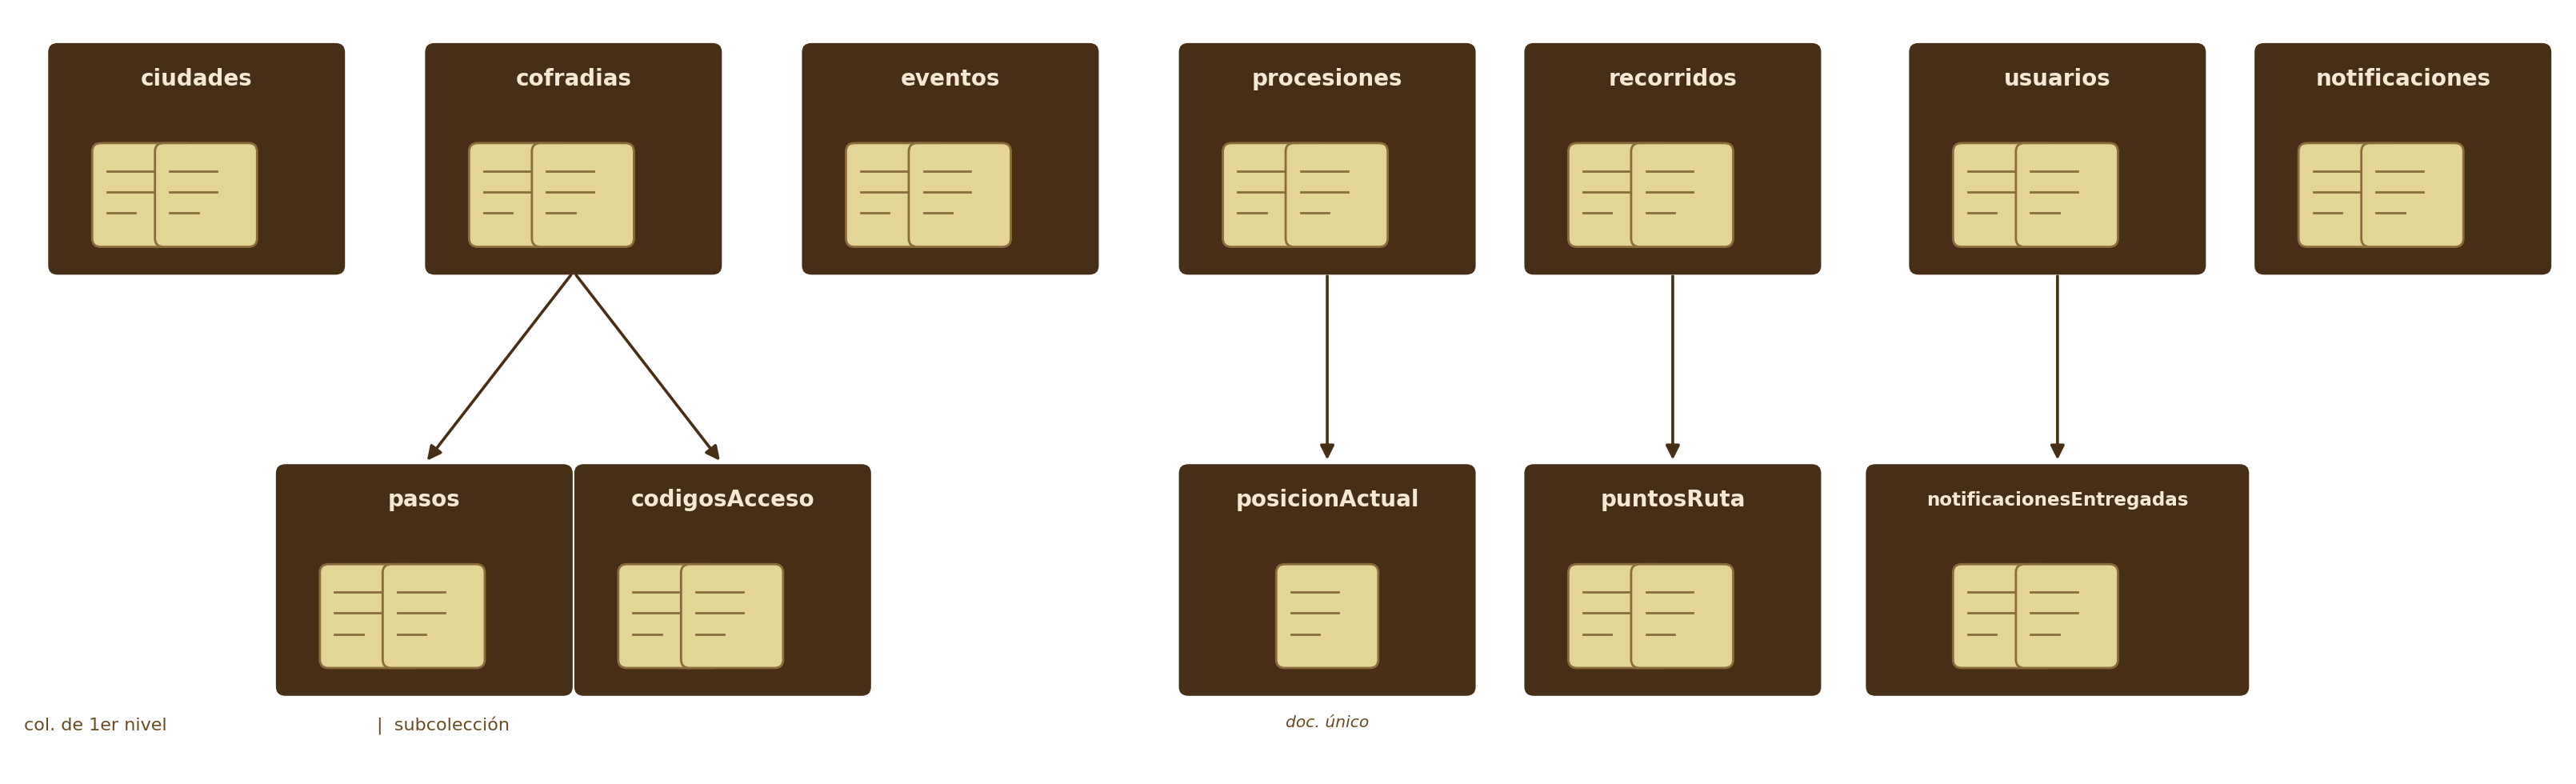
\includegraphics[width=0.9\textwidth]{imagenes/estructura_firestore.png}
    \caption{Estructura de colecciones y subcolecciones de Cloud Firestore}
    \label{fig:EstructuraFirestore}
\end{figure}

El Apéndice~\ref{cap:esquemaBD} recoge, a nivel de campo, el esquema completo de cada colección y subcolección --tipos de dato y referencias incluidas-- para quien necesite el detalle completo de la base de datos.

\subsubsection{Interfaces de usuario}
 
Paralelamente a las decisiones de arquitectura y de base de datos, se ha diseñado en Figma \cite{figma} el conjunto de pantallas del perfil de ciudadano mediante \emph{mockups}\footnote{Mockup: representación visual estática de la interfaz de una aplicación, sin funcionalidad real, utilizada para planificar el diseño antes de su implementación.}, que sirven de referencia visual para la implementación posterior. Se ha optado por diseñar de forma conjunta todas las pantallas del perfil ciudadano, aunque no todas se implementen en esta primera iteración, para garantizar una línea visual coherente desde el principio y evitar rediseños parciales más adelante. De ellas, en esta primera iteración se implementan únicamente la selección de ciudad, la pantalla de inicio y los listados y fichas de detalle de cofradías, procesiones, pasos y eventos; el resto se retoman en la iteración a la que corresponden: el mapa en vivo en la Iteración 2, el modo cofrade y la ubicación compartida del perfil en la Iteración 3, y el calendario, la búsqueda y las preferencias de notificaciones del perfil en iteraciones posteriores.
 
Todas las pantallas comparten una estética oscura con acentos dorados, que evoca la iluminación de cirios y el ambiente nocturno característico de las procesiones, y una barra de navegación inferior fija con cinco secciones (\emph{Inicio}, \emph{Calendario}, \emph{Mapa}, \emph{Buscar} y \emph{Perfil}), que se corresponde directamente con el paquete \texttt{navigation/} descrito en el apartado de arquitectura. Los listados de cofradías, procesiones, pasos y eventos ya no ocupan una sección propia de la barra de navegación, sino que se accede a ellos desde un menú contextual en la pantalla de \emph{Inicio}, tal y como se explica más adelante.
 
La paleta de color se apoya en tonos marrón muy oscuro, casi negro, para el fondo (\texttt{\#1E1008}, \texttt{\#120A06}, \texttt{\#34150E}, \texttt{\#472F17}), dorados como color de acento para títulos, iconos activos y elementos interactivos (\texttt{\#C9A84C}, \texttt{\#9A7D60}), tonos crema para tarjetas y textos secundarios (\texttt{\#F0E0C8}, \texttt{\#E3D595}) y blanco (\texttt{\#FFFFFF}) para el texto principal sobre fondo oscuro; un verde puntual (\texttt{\#37E37E}) se reserva para indicadores de estado, como una procesión en curso. En cuanto a la tipografía, se combinan tres familias: \textbf{Cormorant Garamond}, una serifa elegante, para los títulos, coherente con la estética evocada; \textbf{Lora}, también serifa pero más neutra, para el texto de lectura extensa (historia de una cofradía, descripción de un paso); y \textbf{Sora}, de palo seco, para los elementos de interfaz (botones, etiquetas, barra de navegación), donde interesa más la legibilidad a tamaños pequeños que el carácter estético. Estas decisiones se apoyan, además del criterio propio, en las pautas de \emph{Material Design~3} \cite{materialdesign3}, la guía de diseño de interfaz de Google, en particular en lo relativo al contraste de color, el tamaño mínimo táctil de los elementos interactivos y la estructura de la barra de navegación inferior.
 
\paragraph{Selección de ciudad}
 
Es la primera pantalla que ve cualquier usuario, ya que toda la información de la aplicación (cofradías, procesiones, eventos) está filtrada por la ciudad seleccionada, tal y como se refleja en la colección \texttt{ciudades} descrita en el apartado anterior. El usuario puede buscar su ciudad o elegirla de una lista con el número de procesiones disponibles en cada una.
 
\begin{figure}[H]
    \centering
    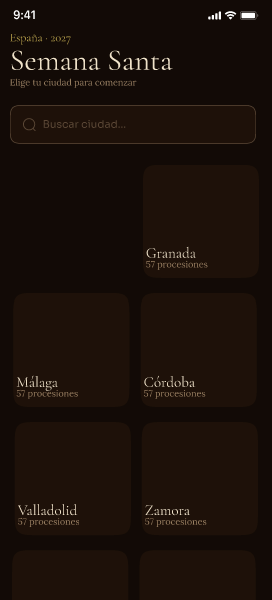
\includegraphics[width=0.45\textwidth]{imagenes/eleguirCiudad.png}
    \caption{Mockup de la pantalla de selección de ciudad}
    \label{fig:mockupCiudad}
\end{figure}
 
\paragraph{Inicio}
 
Muestra la información general del día de Semana Santa seleccionado: un aviso destacado si existe alguna incidencia relevante (por ejemplo, un retraso en el horario de salida), la procesión que está en curso en ese momento si la hay, unas estadísticas generales de la ciudad (número de cofradías, procesiones y nazarenos) y el listado de procesiones y eventos programados para el día, marcando cuáles son favoritos del ciudadano. Desde el menú contextual de esta pantalla (icono \emph{overflow} superior derecho) se accede, además, a los listados independientes de cofradías, procesiones, pasos y eventos.
 
\begin{figure}[H]
    \centering
    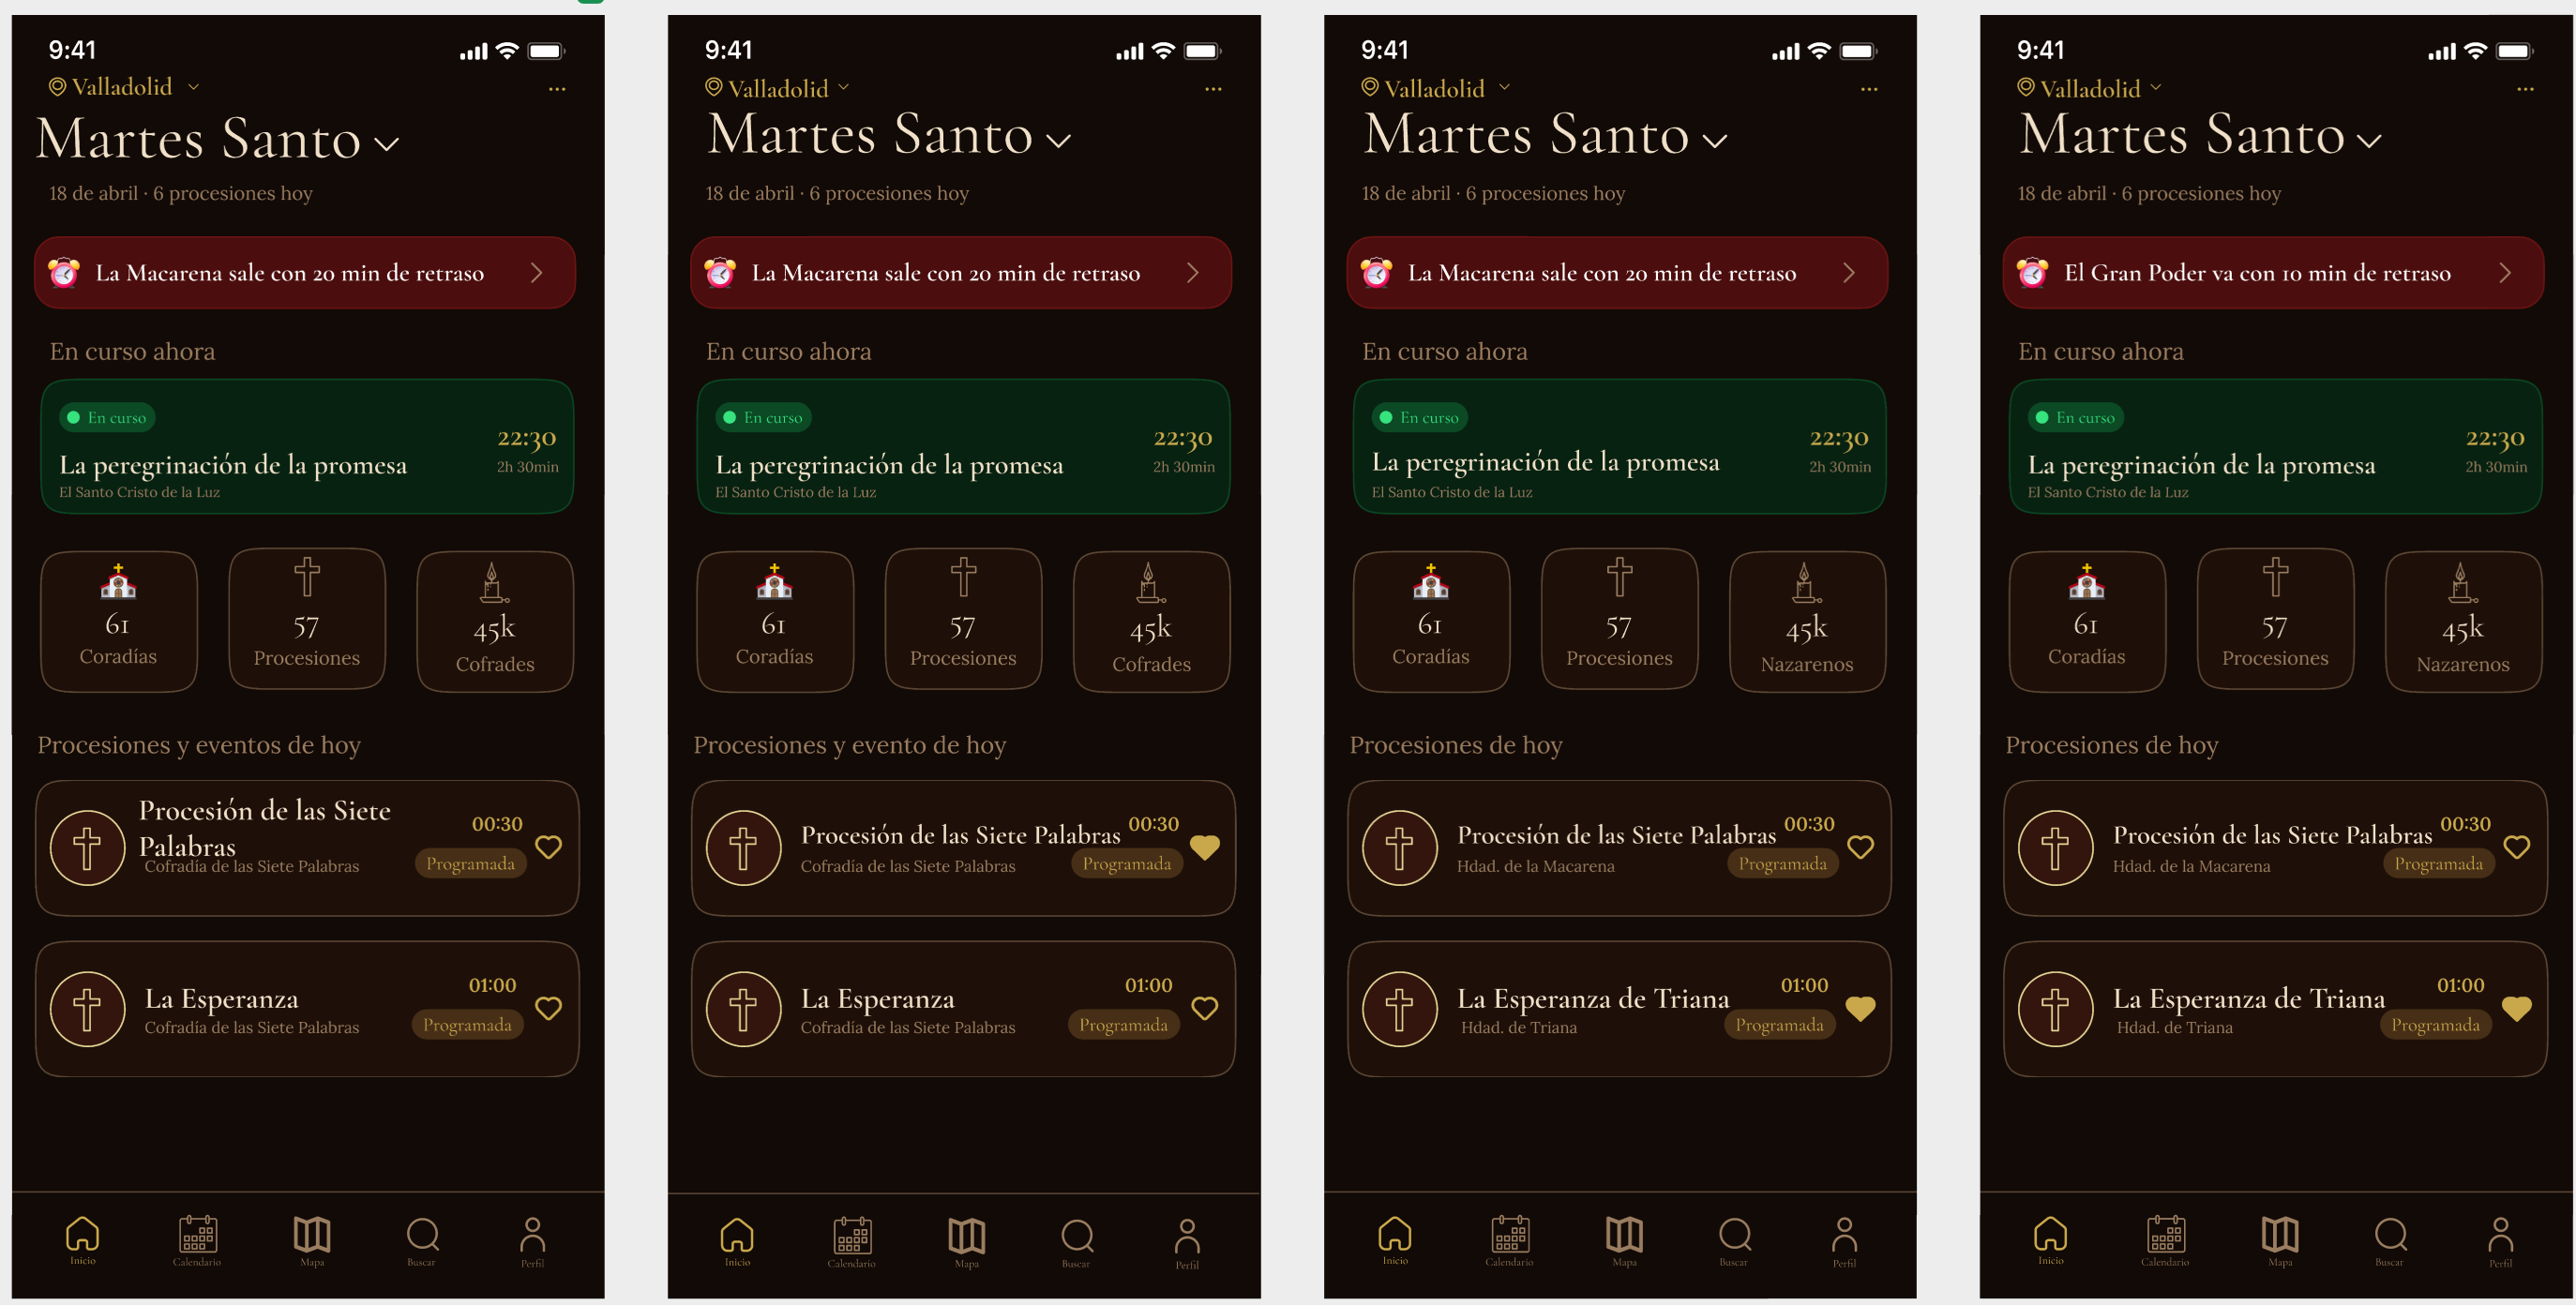
\includegraphics[width=0.9\textwidth]{imagenes/inicioYfav.png}
    \caption{Mockup de la pantalla de inicio: aviso de retraso, procesión en curso, estadísticas y agenda del día}
    \label{fig:mockupInicio}
\end{figure}
 
\paragraph{Calendario}
 
Complementa a la pantalla de inicio permitiendo consultar cualquier otro día de la Semana Santa, no solo el actual. Ofrece dos niveles de detalle: una vista mensual completa, con un indicador en los días que tienen procesiones programadas, y una vista semanal con la agenda del día seleccionado, listando sus procesiones con horario y duración.
 
\begin{figure}[H]
    \centering
    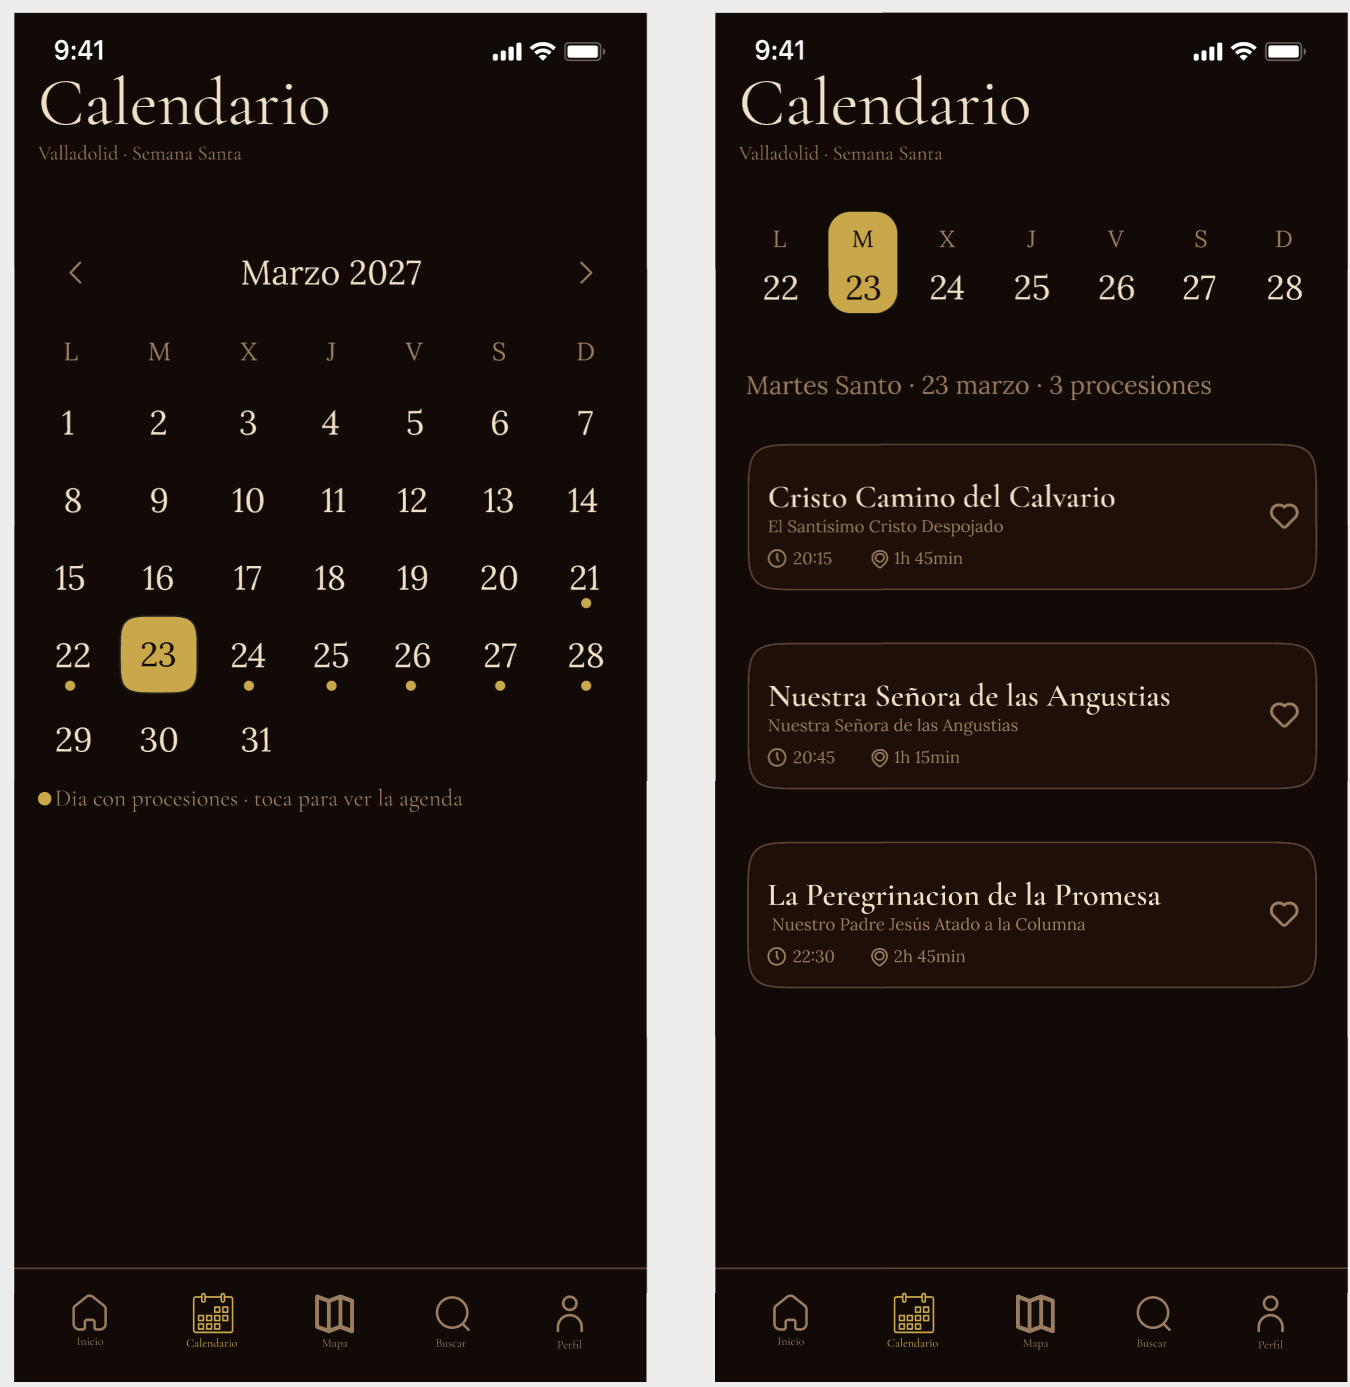
\includegraphics[width=0.9\textwidth]{imagenes/calendario.png}
    \caption{Mockup de la pantalla de calendario: vista mensual y agenda del día seleccionado}
    \label{fig:mockupCalendario}
\end{figure}
 
\paragraph{Listados de cofradías, procesiones, pasos y eventos}
 
Cada uno de estos cuatro elementos del dominio cuenta con su propio listado, accesible desde el menú de la pantalla de Inicio, con buscador propio y sin más información que el nombre de cada elemento, ya que su detalle se consulta accediendo a la ficha correspondiente.
 
\begin{figure}[H]
    \centering
    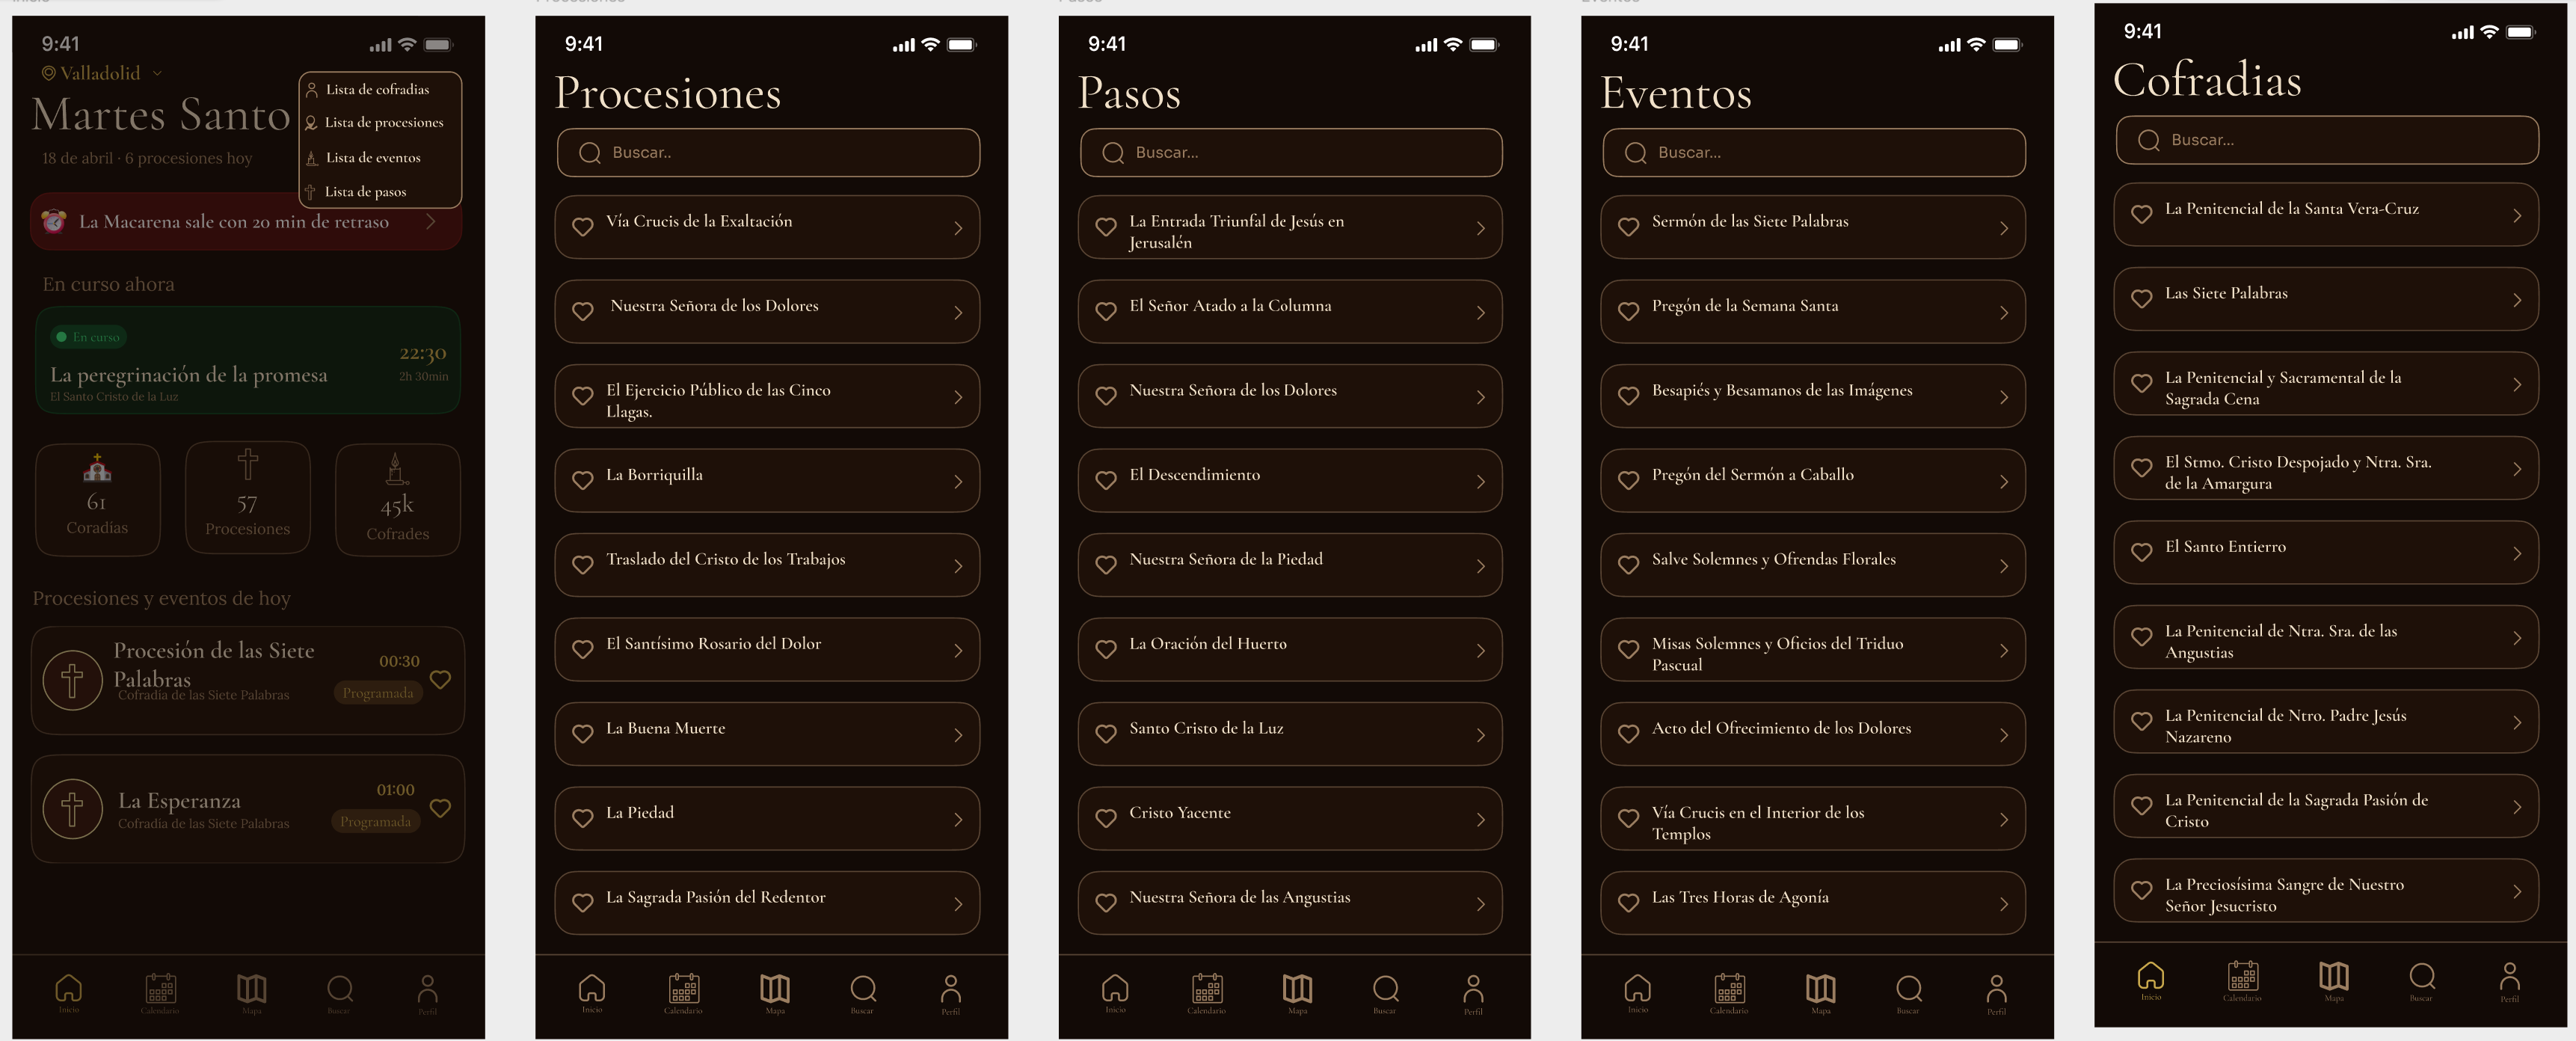
\includegraphics[width=0.95\textwidth]{imagenes/listados.png}
    \caption{Mockup del menú de la pantalla de inicio y de los listados de procesiones, pasos, eventos y cofradías}
    \label{fig:mockupListados}
\end{figure}
 
\paragraph{Detalle de cofradía y de paso}
 
La ficha de una cofradía muestra su historia, su web oficial, las procesiones y el evento que organiza y los pasos que la componen. De forma análoga, la ficha de un paso muestra una imagen, su historia y origen, un análisis artístico y su web oficial, siguiendo la misma estructura visual que la ficha de cofradía para mantener la coherencia del conjunto.
 
\begin{figure}[H]
    \centering
    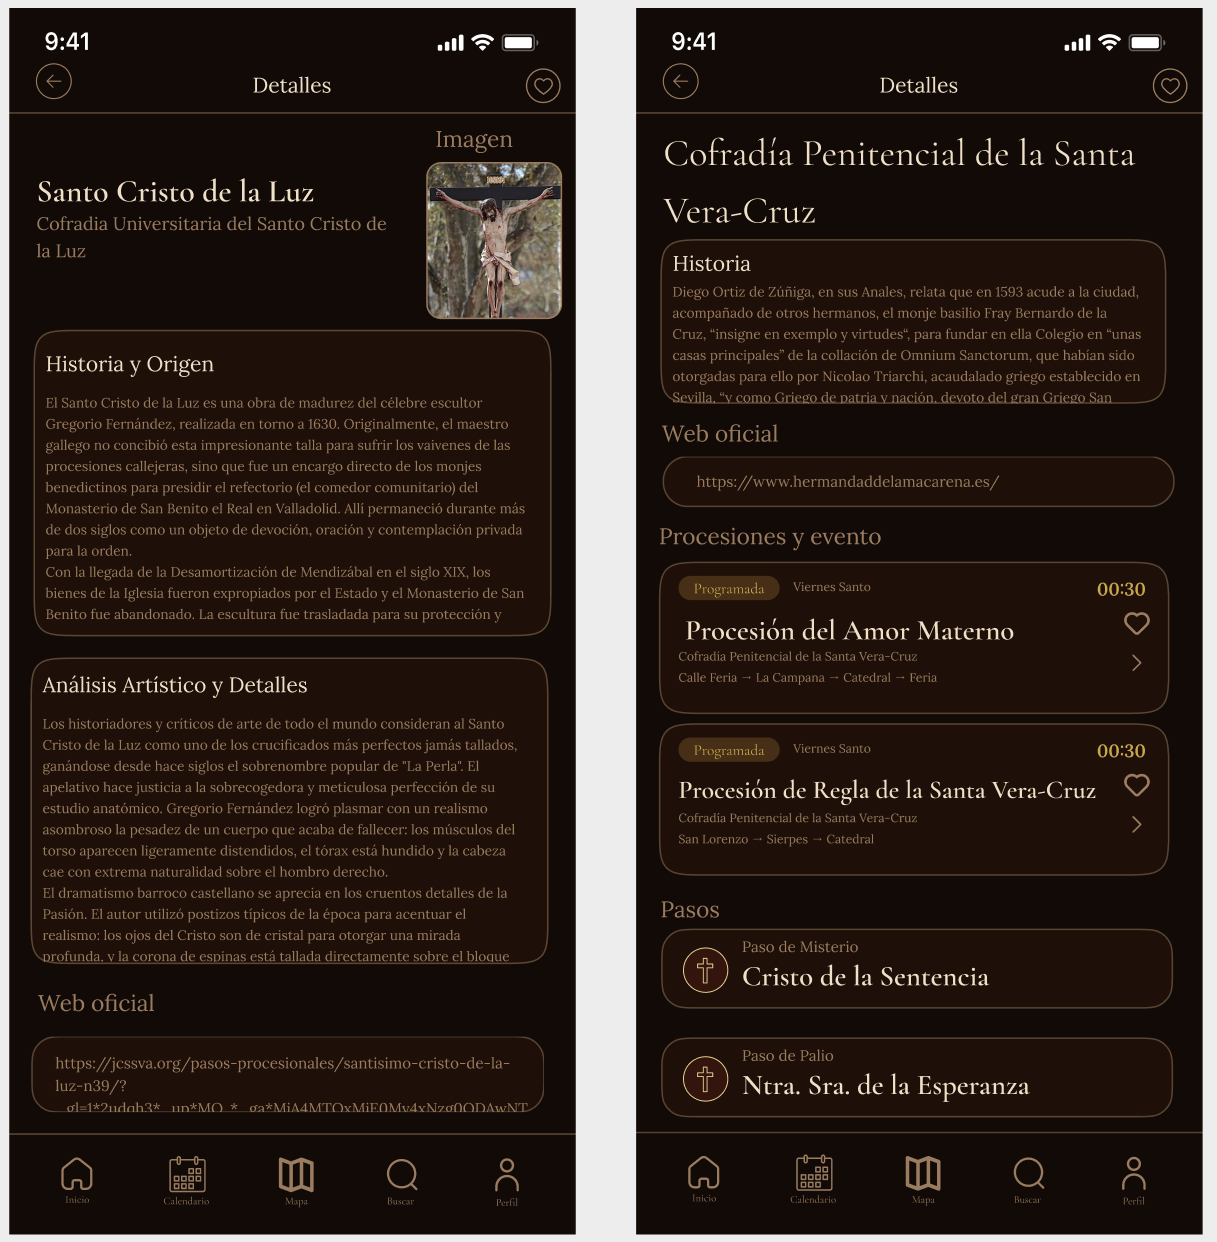
\includegraphics[width=0.9\textwidth]{imagenes/infoPasoyCofradia.png}
    \caption{Mockup del detalle de un paso y de una cofradía}
    \label{fig:mockupDetalleCofradiaPaso}
\end{figure}
 
\paragraph{Detalle de procesión}
 
Muestra el estado de la procesión (programada, en curso o finalizada), su día y hora de salida, duración, número de nazarenos, los pasos que participan en ella y su recorrido sobre un mapa, con un botón de acceso directo al mapa en vivo si la procesión está en curso. Además, de forma similar a la ficha de una cofradía, cada procesión tiene una pantalla de información ampliada con la historia y el origen del desfile.
 
\begin{figure}[H]
    \centering
    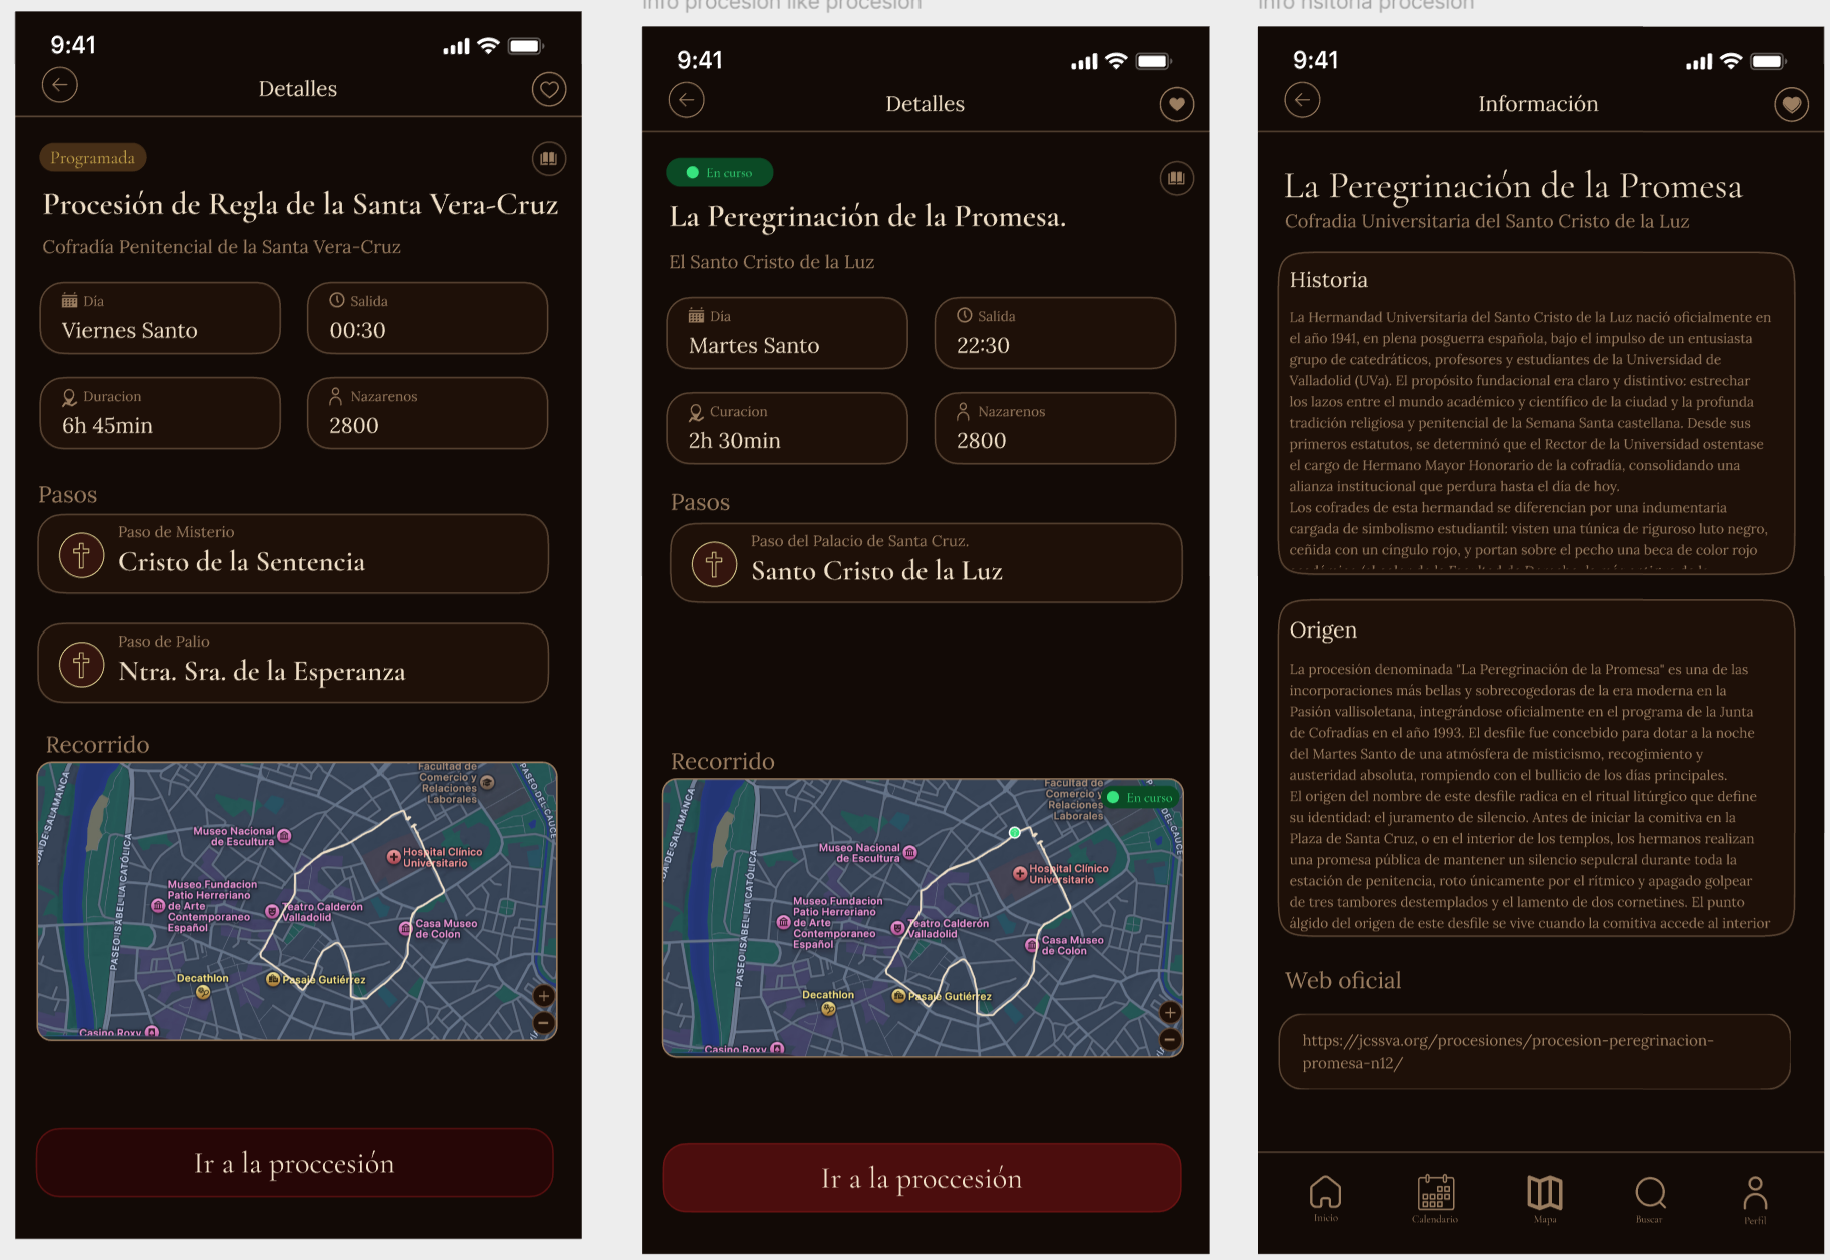
\includegraphics[width=0.95\textwidth]{imagenes/procesionDetalleNuevo.png}
    \caption{Mockup del detalle de una procesión (programada y en curso) y de su información ampliada}
    \label{fig:mockupDetalleProcesion}
\end{figure}
 
\paragraph{Buscar}
 
Permite localizar procesiones, pasos y eventos combinando texto libre con filtros por día de Semana Santa y por estado (programada, en curso o finalizada), mostrando un mensaje cuando ningún resultado cumple los filtros seleccionados. Su funcionalidad se implementa en una iteración posterior.
 
\begin{figure}[H]
    \centering
    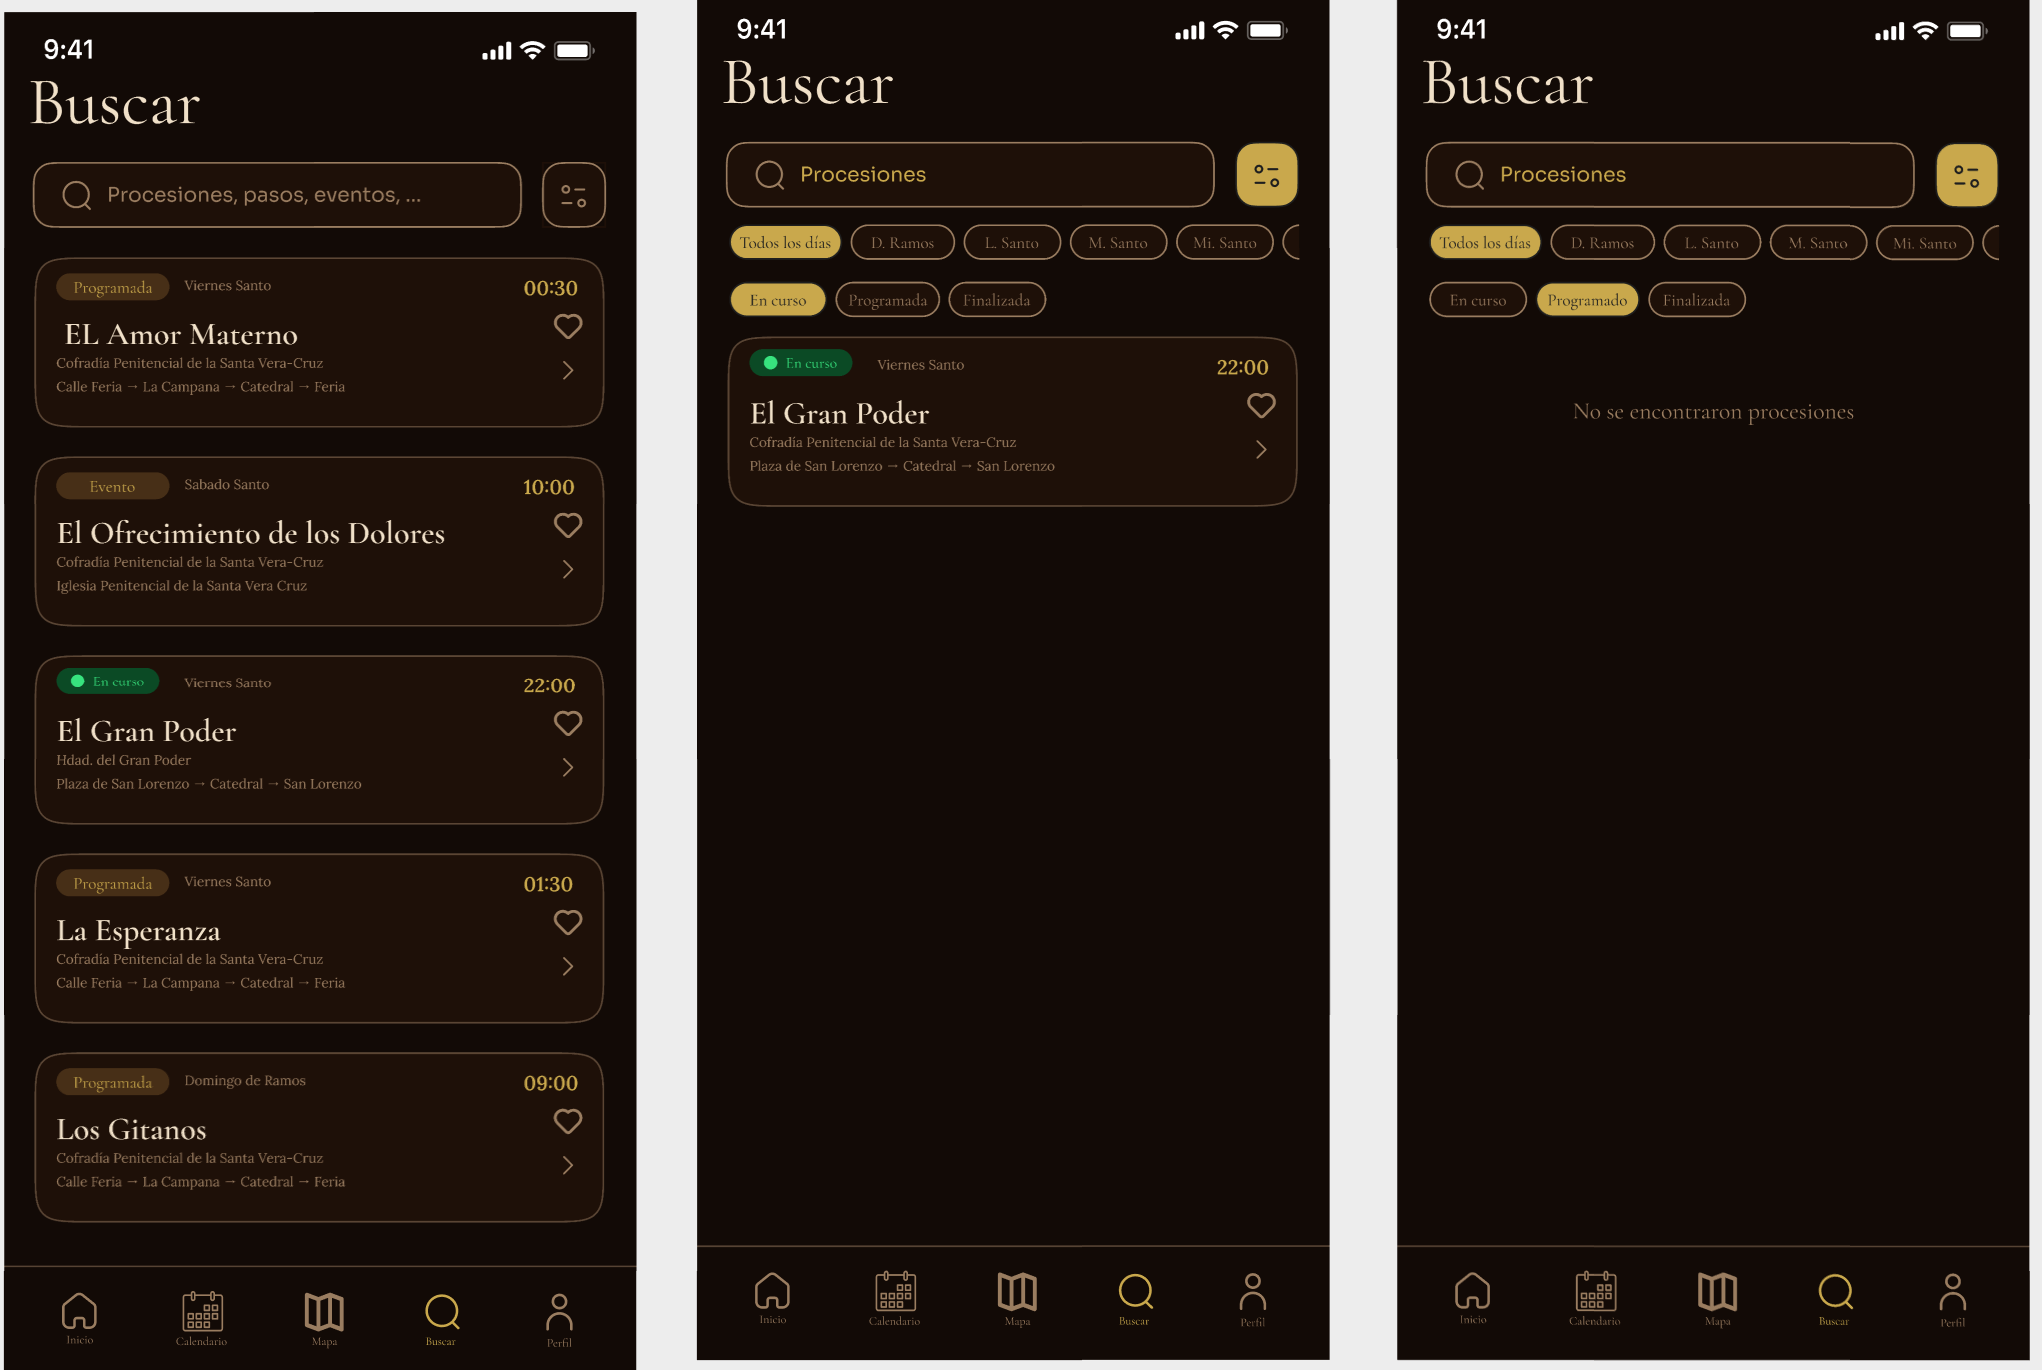
\includegraphics[width=0.9\textwidth]{imagenes/buscaryFiltrar.png}
    \caption{Mockup de la pantalla de búsqueda con filtros por día y estado}
    \label{fig:mockupBuscar}
\end{figure}
 
\paragraph{Mapa en Vivo}
 
Mostrará sobre un mapa de Google Maps la posición en tiempo real de las procesiones en curso y la ubicación del propio ciudadano, junto con un listado de las procesiones actualmente en movimiento desde el que centrar el mapa sobre una de ellas. Se implementa en la Iteración 2.
 
\begin{figure}[H]
    \centering
    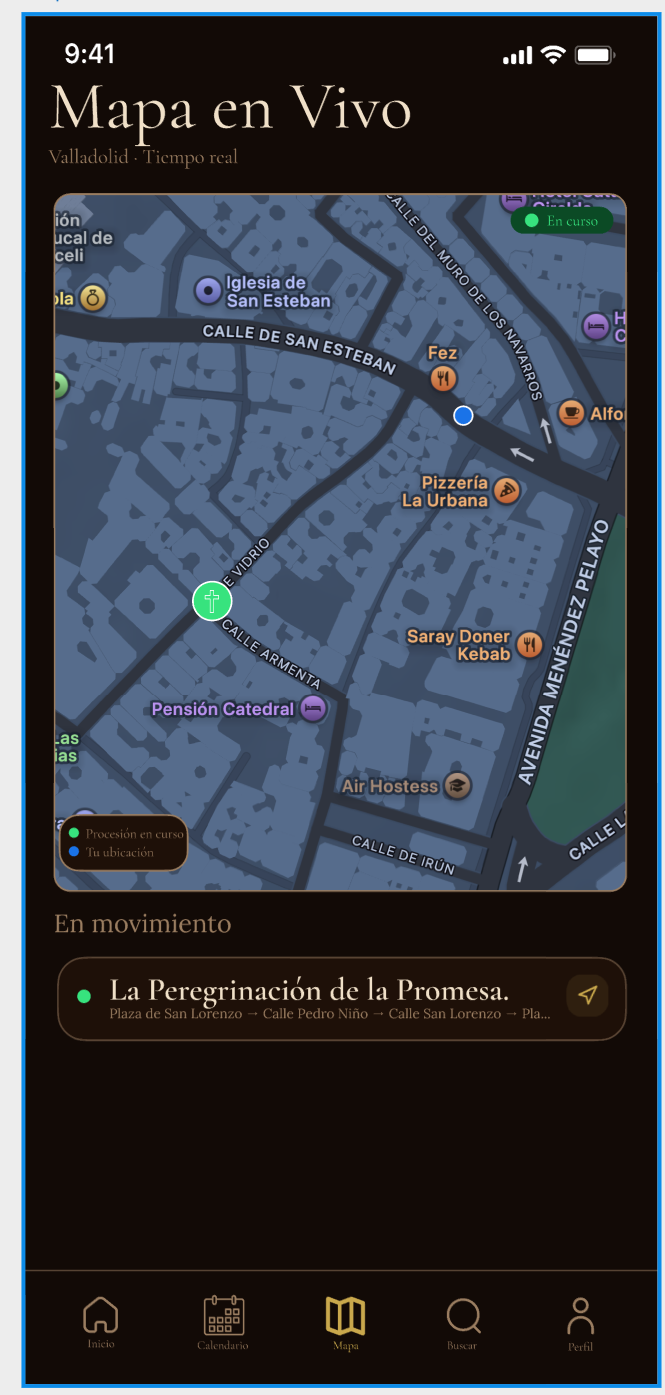
\includegraphics[width=0.45\textwidth]{imagenes/mapaEnVivo.png}
    \caption{Mockup del mapa en vivo}
    \label{fig:mockupMapa}
\end{figure}
 
\paragraph{Perfil}
 
Reúne la ciudad seleccionada y las cofradías/procesiones favoritas del ciudadano, el cambio entre el modo ciudadano y el modo cofrade, y las preferencias de notificaciones (avisos de procesiones en curso, alertas de tráfico y retrasos). En modo cofrade se añade además el botón para activar la ubicación compartida durante una procesión. El cambio de modo y la ubicación compartida se implementan en la Iteración 3; las preferencias de notificaciones, en una iteración posterior.
 
\begin{figure}[H]
    \centering
    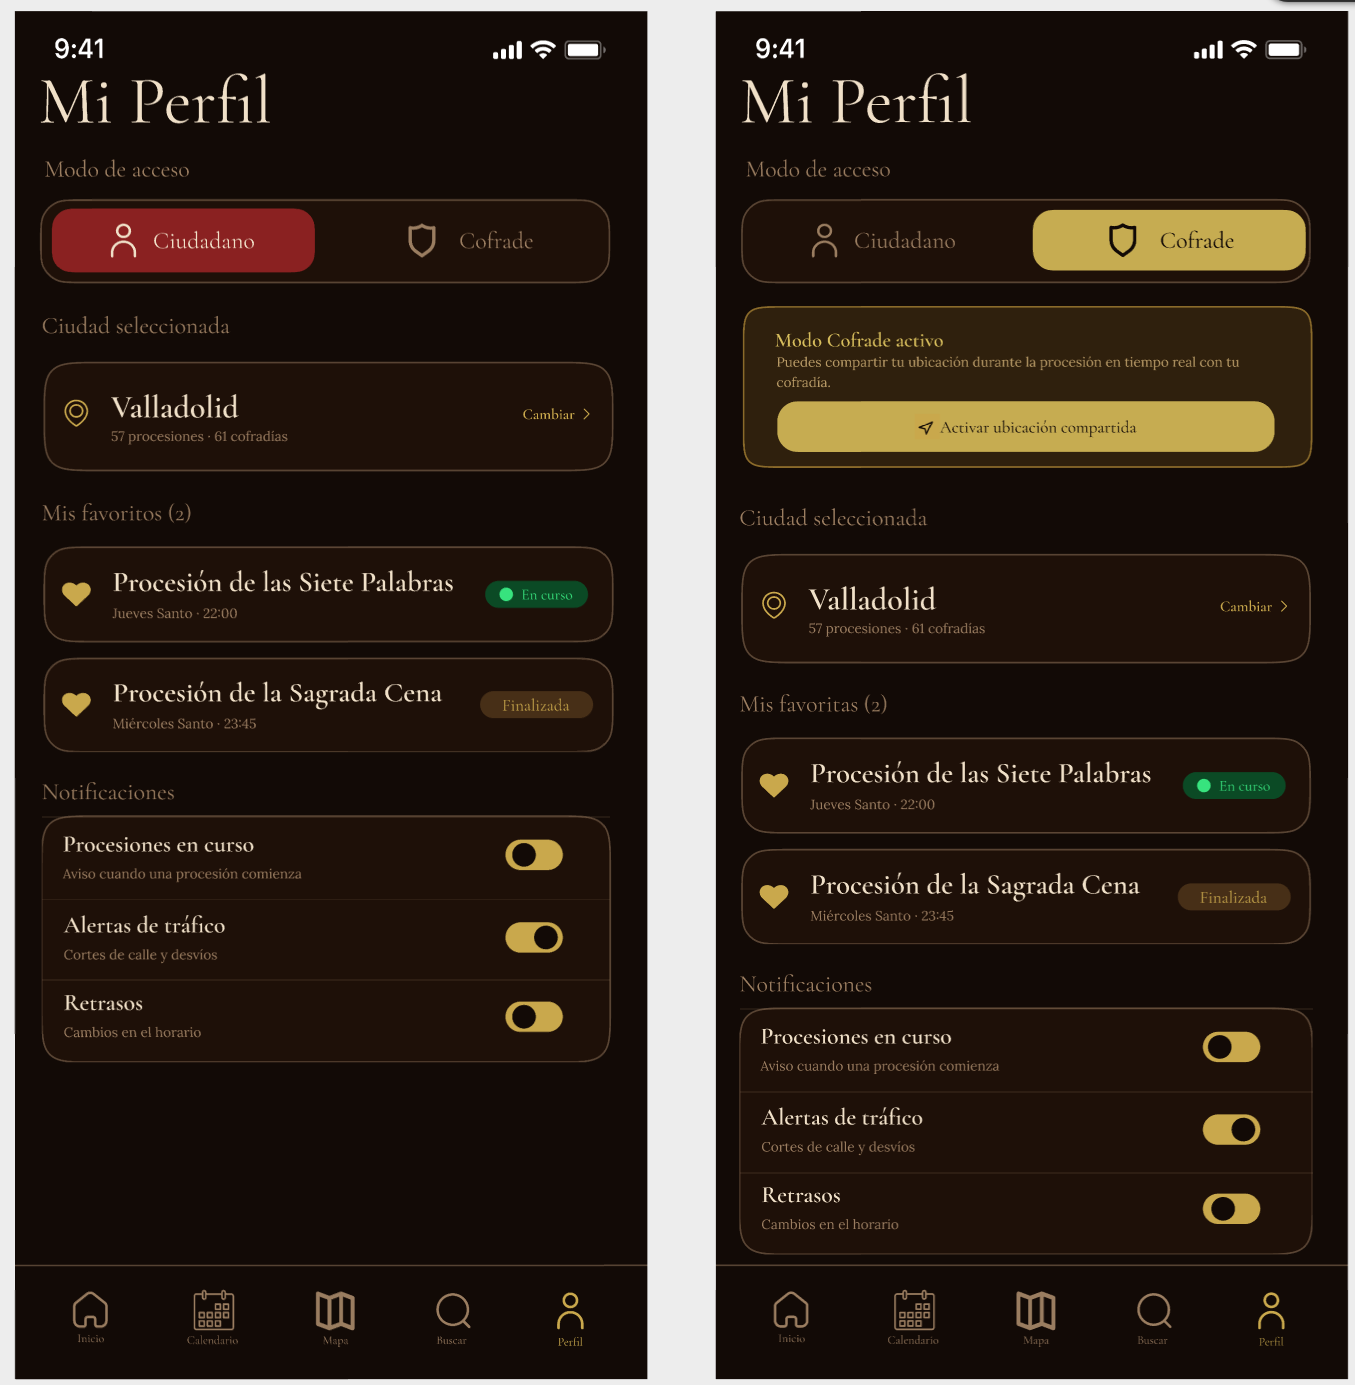
\includegraphics[width=0.9\textwidth]{imagenes/perfiles.png}
    \caption{Mockup de la pantalla de perfil, en modo ciudadano y en modo cofrade}
    \label{fig:mockupPerfil}
\end{figure}
 
\subsubsection{Patrones de diseño}
 
Un patrón de diseño \cite{larman2004} es una solución ya conocida y reutilizable a un problema que se repite con frecuencia en el desarrollo de software; su uso facilita la legibilidad, el mantenimiento y la escalabilidad del código. Para seleccionar los patrones aplicables a este proyecto se han revisado dos TFG previos de la escuela con una arquitectura similar (aplicación móvil apoyada en Firebase), de los que se han descartado los patrones \emph{Builder} y \emph{Abstract Factory}: en Java se justifican porque los constructores de clases no admiten bien parámetros opcionales, pero en JavaScript/TypeScript un objeto literal con esos mismos campos opcionales ya resuelve el mismo problema de forma nativa, y en ningún punto del sistema es necesario intercambiar familias completas de implementaciones. Los siete patrones finalmente aplicados son los siguientes:
 
\begin{itemize}
    \item \textbf{Singleton}: patrón que garantiza que una clase tenga una única instancia en toda la aplicación y un punto de acceso global a ella, evitando crear varias copias innecesarias. En este proyecto, la inicialización del SDK de Firebase (\texttt{firebase/config}) se realiza una única vez y esa misma instancia se reutiliza en el resto de la aplicación.
    \item \textbf{Repository}: patrón que separa la lógica de acceso a los datos del resto de la aplicación, ocultando los detalles de cómo y dónde se almacenan. La capa \texttt{services} es la única parte del código que conoce el SDK de Firebase; el resto de la aplicación solo invoca funciones como \texttt{procesionService.} \texttt{obtenerActivas(ciudadId)}, sin saber que por detrás se está consultando Firestore. Esto facilitaría cambiar de proveedor de backend en el futuro (línea de trabajo futuro, Sección~\ref{cap:trabajo_futuro}) sin modificar ninguna pantalla.
    \item \textbf{Observer}: patrón en el que uno o varios elementos (``observadores'') se suscriben a los cambios de otro elemento y son notificados automáticamente cuando este cambia, en lugar de tener que preguntar repetidamente. Los \emph{listeners} de Firestore (\texttt{onSnapshot}) funcionan así: notifican a la interfaz cada vez que cambia la posición de una procesión o llega una notificación nueva.
    \item \textbf{Factory Method}: patrón que centraliza en una única función la creación de un objeto, delegando en ella la decisión de qué variante concreta construir. El dominio distingue \texttt{Aviso} y \texttt{Alerta} como subtipos de \texttt{Notificacion} (Figura~\ref{fig:DiagramDomain}); una función fábrica construye el objeto correcto según los campos \texttt{tipoAlerta} y \texttt{fechaExpiracion} antes de guardarlo en Firestore.
    \item \textbf{Context/Provider}: convención propia de React (no un patrón GoF\footnote{GoF (\emph{Gang of Four}): apodo con el que se conoce a los cuatro autores del libro \emph{Design Patterns} \cite{gof} (1994), que popularizó el catálogo clásico de patrones de diseño orientado a objetos (Singleton, Observer, Factory Method, entre otros).} clásico) que permite exponer un dato o estado a cualquier pantalla de la aplicación sin tener que pasarlo manualmente de componente en componente. \texttt{AuthContext} y \texttt{LocationContext} exponen así el usuario autenticado y los permisos de ubicación a cualquier pantalla que los necesite.
    \item \textbf{Facade}: patrón que ofrece una única función sencilla como punto de entrada a una operación que, por detrás, involucra varios pasos o subsistemas distintos. El caso de uso ``Compartir ubicación durante procesión'' (RF-15) esconde tras la llamada \texttt{geoService.iniciarCompartirUbicacion} \texttt{(procesionId)} la solicitud de permiso de GPS, la escritura periódica en Firestore y la gestión de una posible pérdida de conexión.
    \item \textbf{Adapter}: patrón que convierte el formato de datos de un sistema externo al formato interno que espera la aplicación, permitiendo que ambos ``encajen'' sin modificar ninguno de los dos. Las notificaciones \emph{push} de Firebase Cloud Messaging llegan con un formato plano (título, cuerpo, y un mapa de texto), distinto del modelo interno tipado \texttt{Alerta}/\texttt{Aviso}; una función adaptadora convierte ese \emph{payload} recibido al modelo de dominio antes de utilizarlo en la aplicación.
\end{itemize}
 
\subsection{Implementacion}
 
\subsection{Pruebas}